\documentclass[11pt,a4paper]{article}
\usepackage[utf8]{inputenc}
\usepackage[T1]{fontenc}
\usepackage[french]{babel}
\usepackage{geometry}
\usepackage{graphicx}
\usepackage{booktabs}
\usepackage{amsmath}
\usepackage{hyperref}
\geometry{margin=2.4cm}

\title{Recodage de Ian Wright\\\large Implicit Microfoundations for Macroeconomics}
\author{Recodage Python: numpy, scipy, matplotlib}
\date{1 juillet 2026}

\begin{document}
\maketitle

\section{Objectif}

L'article propose un modèle multi-agents minimal de relations capitalistes. Les agents possèdent de la monnaie, peuvent employer ou être employés, dépensent aléatoirement, génèrent un revenu de firme et reçoivent ou paient des salaires. Le recodage vise à reproduire les figures 1 à 14: classes, tailles de firme, démises, durées de vie, croissance, profits, PIB, récessions, revenus, richesse et sensibilité aux conditions initiales.

\section{Implémentation}

Le script \texttt{../recoding.py} suit l'appendice Mathematica de l'article. Chaque mois, $N$ agents sont tirés avec remise; pour chaque agent sont appliquées les règles de hiring, effective demand, firm income, wage payment and firing. Les sorties sont les figures dans \texttt{../figures/} et le fichier \texttt{../results/summary.json}.

La suite de figures finale utilise $N=1000$, 130 années simulées dont 30 de burn-in. Une campagne séparée, \texttt{../statistical\_analysis.py}, répète cinq fois chaque jeu de paramètres à cette même échelle. Les résultats agrégés sont dans \texttt{../results/statistical\_summary.json}.

\section{Résultats numériques}

\begin{table}[h]
\centering
\begin{tabular}{lrr}
\toprule
Quantité & Reproduction & Valeur article \\
\midrule
Travailleurs moyens & 47.0\% [46.3,47.7] & env. 64.6\% \\
Capitalistes moyens & 4.70\% [4.51,4.89] & env. 16.9\% \\
Chômeurs moyens & 48.3\% [47.6,49.0] & env. 18.5\% \\
Exposant taille de firme $\alpha$ & 0.584 [0.581,0.587] & env. 0.98 \\
Démises par mois & 32.7 [31.7,33.8] & env. 52 \\
Profit médian & 18.8\% [17.4,20.2] & mode env. 32.5\% \\
Wage share moyen & 0.805 [0.799,0.810] & env. 0.6 \\
\bottomrule
\end{tabular}
\caption{Comparaison synthétique. Reproduction: moyenne et IC 95\% sur cinq runs à $N=1000$.}
\end{table}

\begin{figure}[h]
\centering
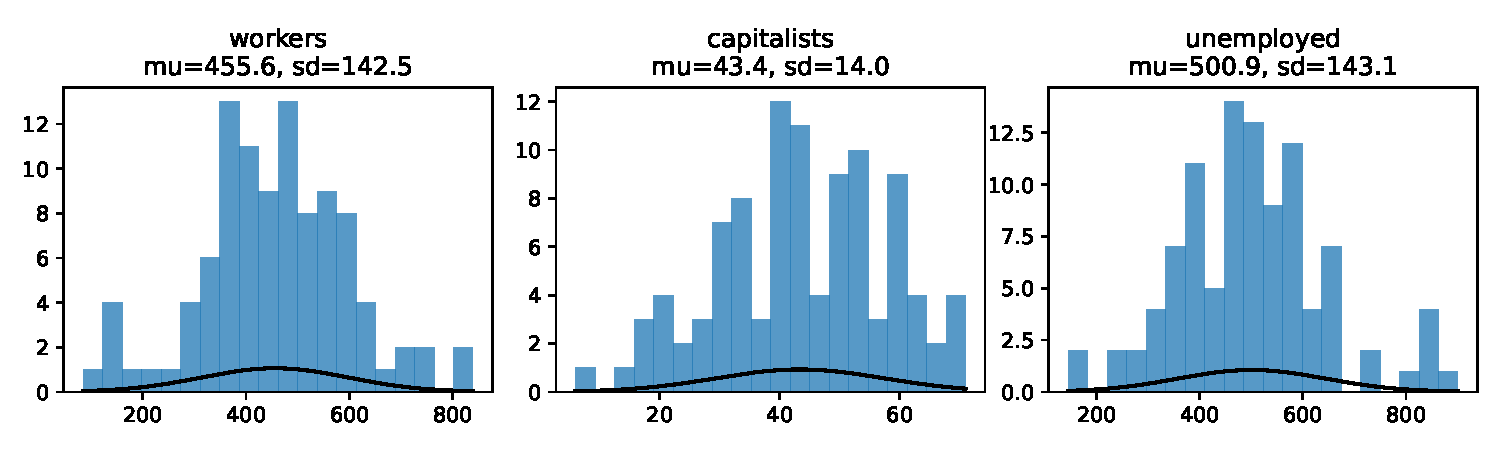
\includegraphics[width=.92\linewidth]{../figures/figure1_class_sizes.pdf}
\caption{Distribution des tailles de classes.}
\end{figure}

\begin{figure}[h]
\centering
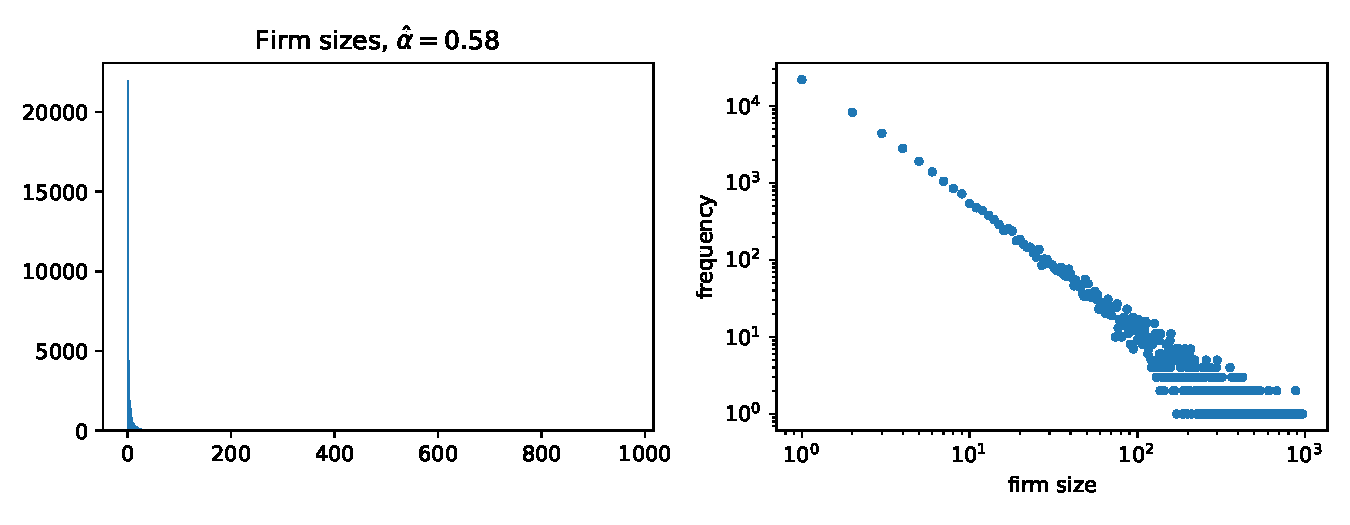
\includegraphics[width=.92\linewidth]{../figures/figure2_firm_sizes.pdf}
\caption{Distribution des tailles de firme.}
\end{figure}

\begin{figure}[h]
\centering
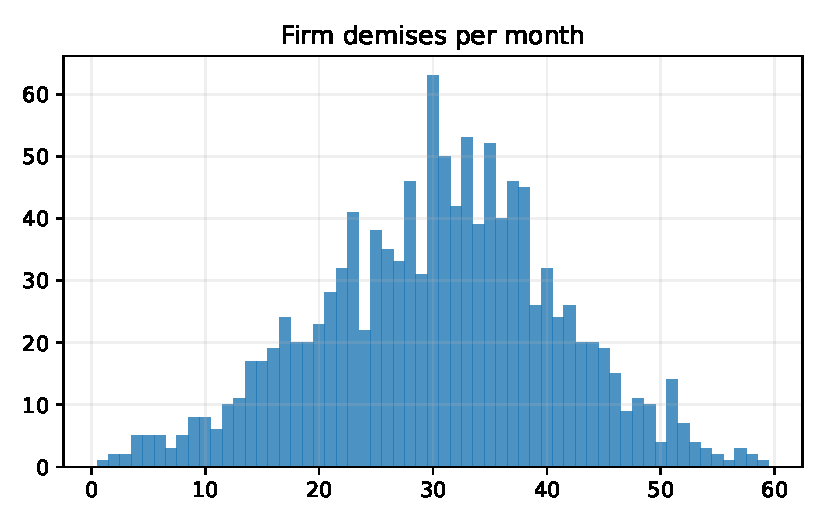
\includegraphics[width=.92\linewidth]{../figures/figure3_demises.pdf}
\caption{Démises de firmes par mois.}
\end{figure}

\begin{figure}[h]
\centering
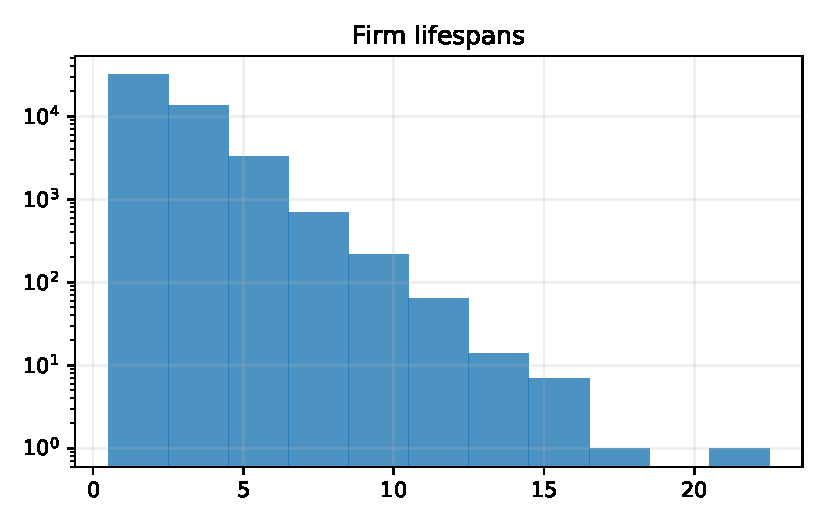
\includegraphics[width=.92\linewidth]{../figures/figure4_lifespans.pdf}
\caption{Durées de vie des firmes.}
\end{figure}

\begin{figure}[h]
\centering
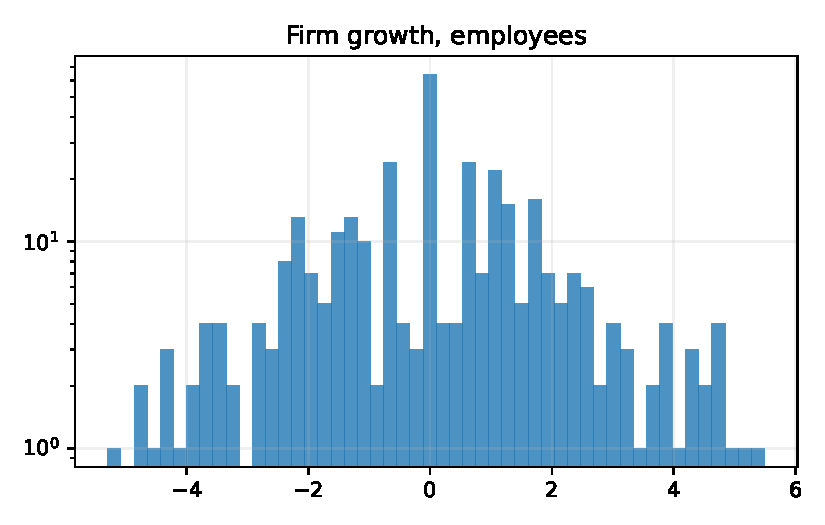
\includegraphics[width=.92\linewidth]{../figures/figure5_growth_employees.pdf}
\caption{Croissance des firmes mesurée par employés.}
\end{figure}

\begin{figure}[h]
\centering
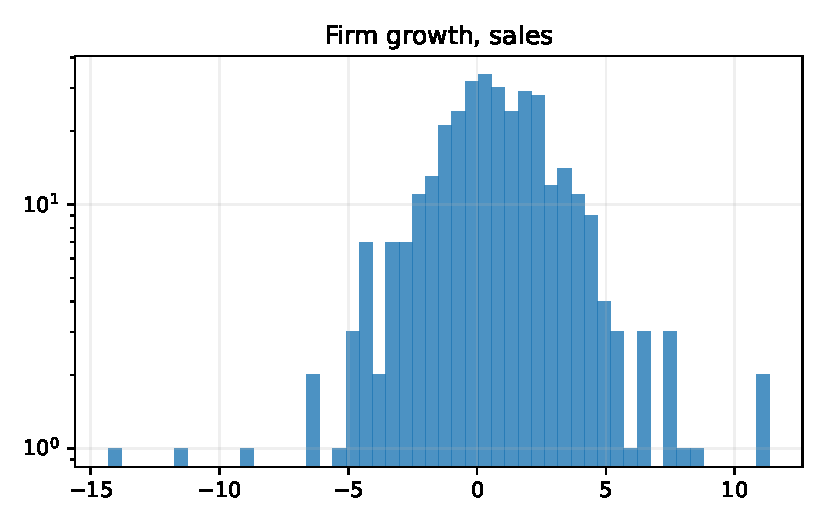
\includegraphics[width=.92\linewidth]{../figures/figure6_growth_sales.pdf}
\caption{Croissance des firmes mesurée par ventes.}
\end{figure}

\begin{figure}[h]
\centering
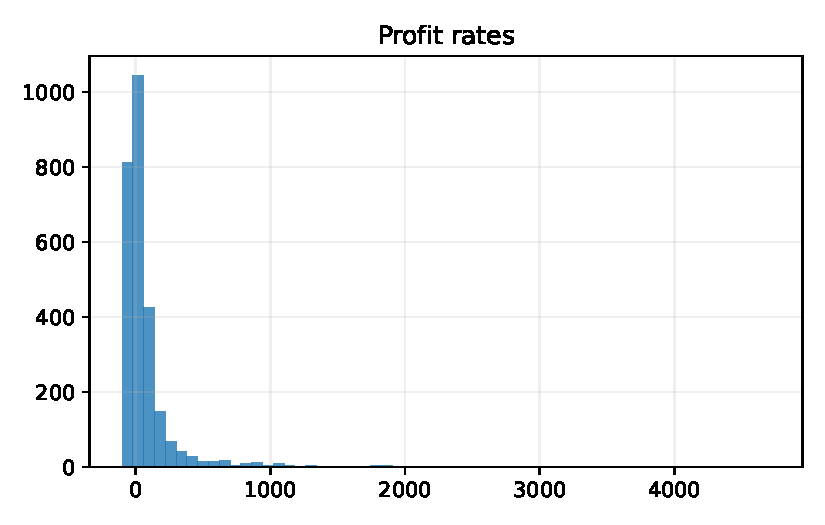
\includegraphics[width=.75\linewidth]{../figures/figure7_profit_rates.pdf}
\caption{Taux de profit.}
\end{figure}

\begin{figure}[h]
\centering
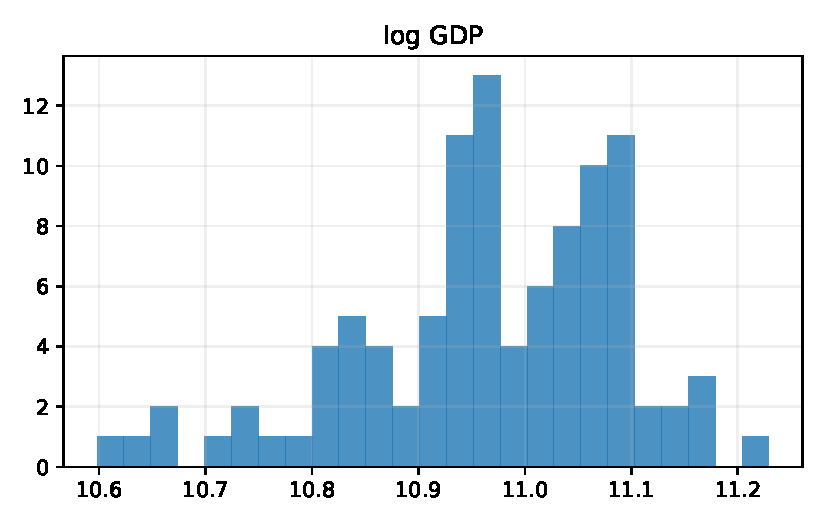
\includegraphics[width=.75\linewidth]{../figures/figure8_log_gdp.pdf}
\caption{Logarithme du PIB.}
\end{figure}

\begin{figure}[h]
\centering
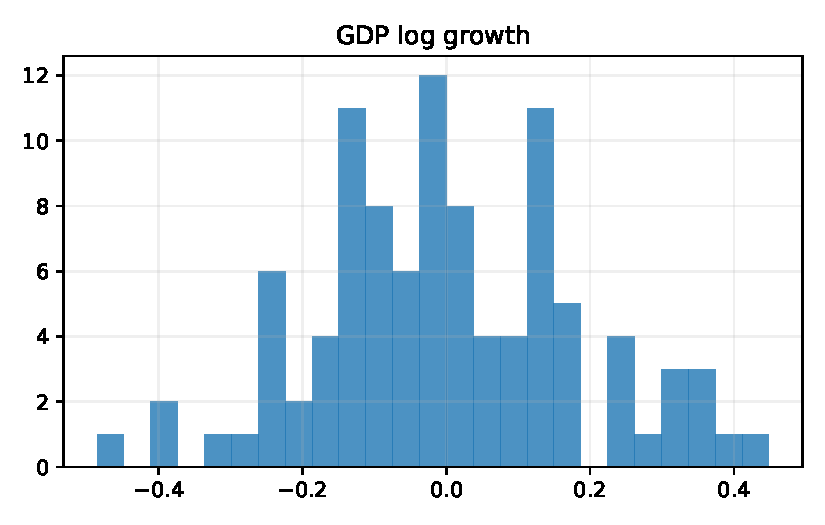
\includegraphics[width=.75\linewidth]{../figures/figure9_gdp_growth.pdf}
\caption{Croissance logarithmique du PIB.}
\end{figure}

\begin{figure}[h]
\centering
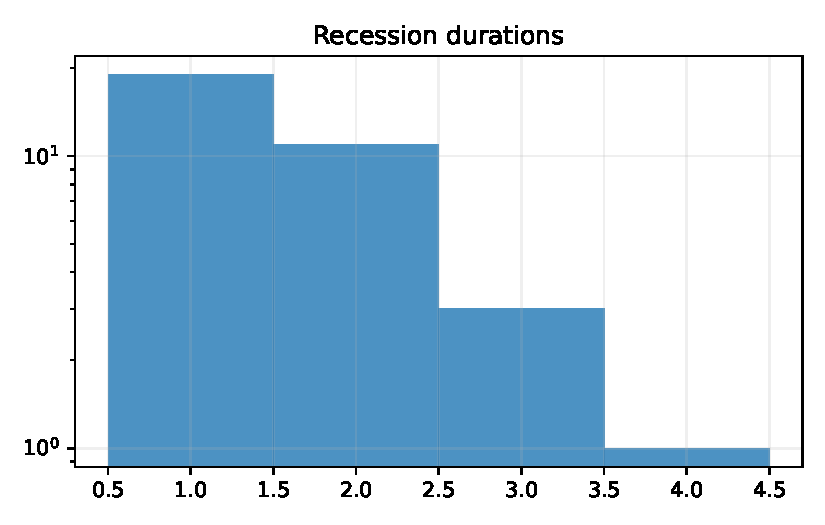
\includegraphics[width=.75\linewidth]{../figures/figure10_recessions.pdf}
\caption{Durées de récessions.}
\end{figure}

\begin{figure}[h]
\centering
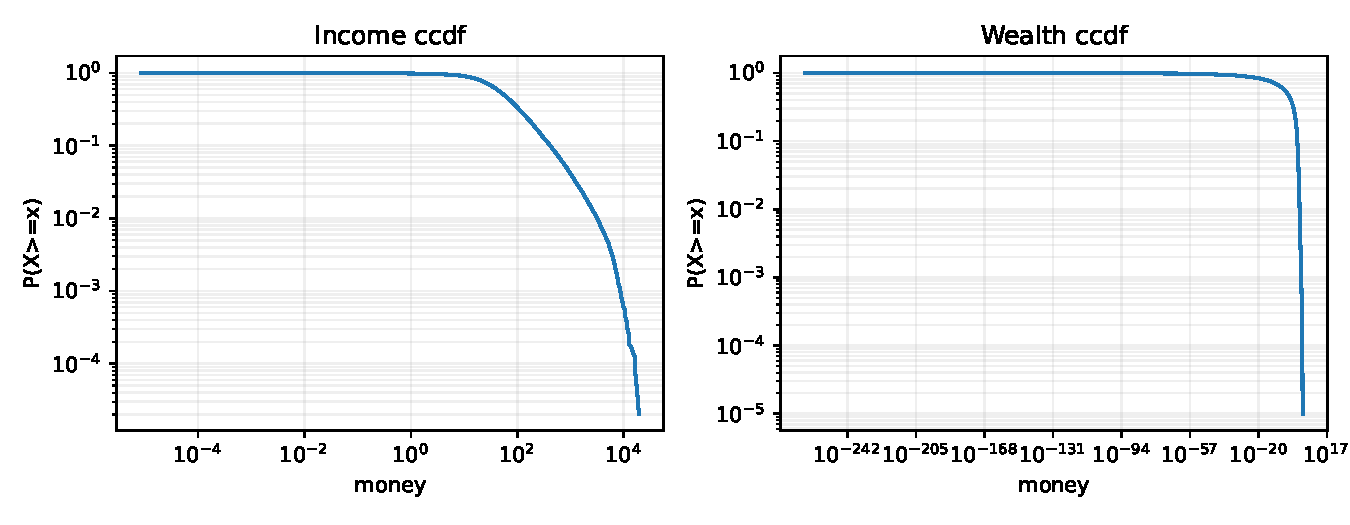
\includegraphics[width=.92\linewidth]{../figures/figure11_12_income_wealth.pdf}
\caption{CCDF des revenus et des richesses monétaires.}
\end{figure}

\begin{figure}[h]
\centering
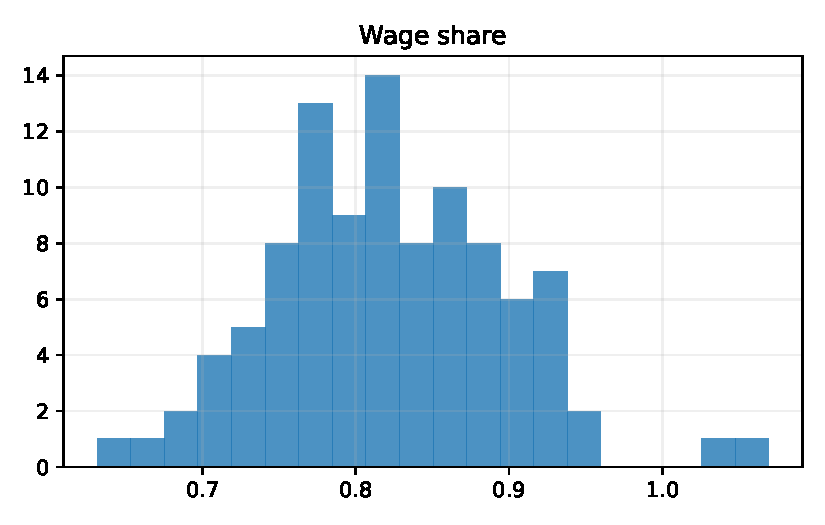
\includegraphics[width=.75\linewidth]{../figures/figure13_wage_share.pdf}
\caption{Part salariale.}
\end{figure}

\begin{figure}[h]
\centering
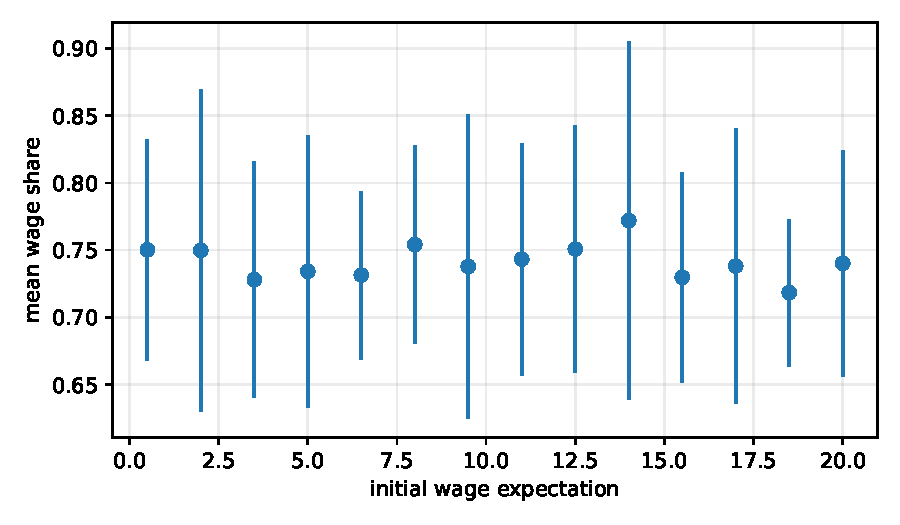
\includegraphics[width=.75\linewidth]{../figures/figure14_wage_seed_sensitivity.pdf}
\caption{Sensibilité de la part salariale à l'attente salariale initiale.}
\end{figure}

\section{Analyse statistique multi-runs et sensibilité}

La campagne lourde comporte cinq runs indépendants de 130 années, dont 30 de burn-in, pour cinq jeux de paramètres à $N=1000$: le cas publié $(m_0,\eta_0)=(10,10)$, deux attentes salariales initiales $\eta_0\in\{5,20\}$ et deux dotations monétaires initiales $m_0\in\{5,20\}$.

\begin{figure}[h]
\centering
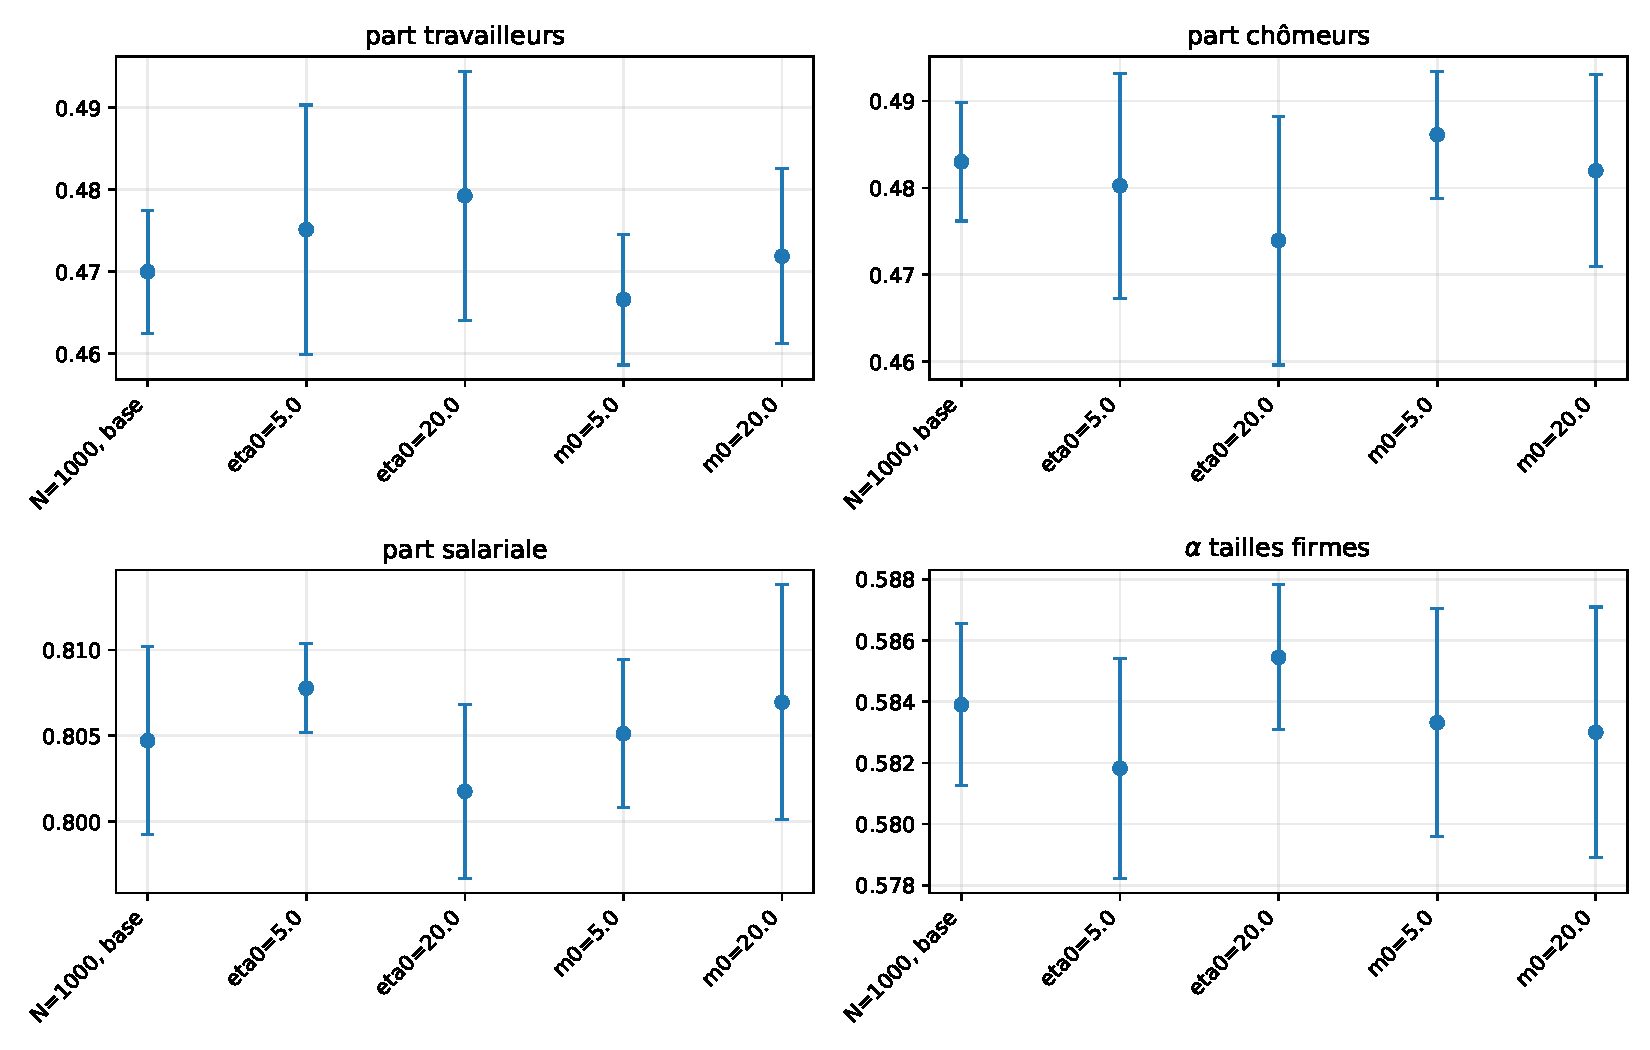
\includegraphics[width=.95\linewidth]{../figures/stat_csa_parameter_sweep.pdf}
\caption{Moyennes et intervalles de confiance à 95\% sur cinq runs par jeu de paramètres.}
\end{figure}

\begin{table}[h]
\centering
\begin{tabular}{lrrrr}
\toprule
Paramètres & travailleurs & chômeurs & wage share & $\alpha$ firmes \\
\midrule
base $(10,10)$ & 0.470 [0.463,0.477] & 0.483 [0.476,0.490] & 0.805 [0.799,0.810] & 0.584 [0.581,0.587] \\
$\eta_0=5$ & 0.475 [0.460,0.490] & 0.480 [0.467,0.493] & 0.808 [0.805,0.810] & 0.582 [0.578,0.585] \\
$\eta_0=20$ & 0.479 [0.464,0.494] & 0.474 [0.460,0.488] & 0.802 [0.797,0.807] & 0.585 [0.583,0.588] \\
$m_0=5$ & 0.467 [0.459,0.475] & 0.486 [0.479,0.493] & 0.805 [0.801,0.809] & 0.583 [0.580,0.587] \\
$m_0=20$ & 0.472 [0.461,0.483] & 0.482 [0.471,0.493] & 0.807 [0.800,0.814] & 0.583 [0.579,0.587] \\
\bottomrule
\end{tabular}
\caption{Résultats agrégés des 25 runs lourds.}
\end{table}

Les intervalles de confiance se recouvrent largement pour tous les paramètres testés. L'insensibilité aux conditions initiales revendiquée par l'article est donc confirmée: doubler ou diviser par deux l'attente salariale et la dotation monétaire initiales ne modifie pas significativement le régime stationnaire.

Cette robustesse renforce toutefois l'infirmation quantitative. Le cas de base donne systématiquement environ 47\% de travailleurs, 4.7\% de capitalistes et 48.3\% de chômeurs, très loin des 64.6\%, 16.9\% et 18.5\% publiés. De même, la part salariale reste autour de 0.805 et l'exposant de taille de firme autour de 0.584. Les écarts sont beaucoup plus grands que les incertitudes inter-runs; ils ne peuvent donc pas être expliqués par la graine ou le transitoire.

\section{Points insuffisamment décrits et choix faits}

\begin{itemize}
  \item L'appendice Mathematica est la spécification principale, mais il ne précise pas la procédure de fitting; j'ai donc reproduit des diagnostics graphiques et des estimateurs simples.
  \item La fonction \texttt{SelectEmployer} de l'appendice exclut l'agent actif via \texttt{NotMe}; j'ai conservé ce choix.
  \item La collecte exacte des statistiques après convergence n'est pas donnée avec une durée de burn-in précise. J'ai utilisé 30 années de burn-in et 100 années utiles pour chaque run lourd.
  \item La figure 14 balaie de nombreux seeds à $N=100$ comme dans le papier. La nouvelle campagne de sensibilité complète ce diagnostic avec 25 runs à $N=1000$ et durée longue.
\end{itemize}

\section{Conclusion}

La reproduction confirme qualitativement plusieurs formes: queues lourdes des tailles de firme, asymétrie des profits, récessions courtes et distributions de revenus/richesses à longue queue. Elle confirme également l'insensibilité du régime stationnaire aux conditions initiales. En revanche, les 25 runs lourds infirment quantitativement les valeurs publiées de classes, de part salariale et d'exposant de taille de firme: les écarts sont stables et très supérieurs aux intervalles de confiance. La cause la plus plausible est une convention d'implémentation ou de mesure non explicitée malgré l'appendice Mathematica, plutôt qu'un manque de durée ou une fluctuation aléatoire.

\end{document}
